\chapter{Fake rate of photon detection}
\label{ch:rate}

In chapter~\ref{ch:snr} we measured the signal to noise ratio after filtering.
The point of using the SNR is expressing the signal height relative to the
width of the noise distribution, because the threshold required to reject noise
with a fixed probability is proportional to that scale. So it is convenient to
express the threshold relative to the same scale, and check it is less than the
SNR so that signals are not selected away.

\marginpar{The title is misleading, since ``fake rate of \emph{photon}
detection'' would imply that DCR is included.}

Even assuming that the noise is gaussian, the probability that a random
fluctuation gets over the threshold is not given simply by computing the
survival function (i.e.\ the integral to $+\infty$) of the gaussian
distribution at the threshold.

More precisely, the probability that any given sample is above the threshold is
given by such integral. What we need, however, is the \emph{rate} of threshold
\emph{crossings}. The noise is not white, but even if it was, after applying
the filter, which combines linearly many input samples for each output sample,
the waveform is autocorrelated at least up to the length of the filter.
Intuitively, if a smooth function crosses a threshold, it takes some time to go
down before it can cross the threshold again.

Since the first stage filtering procedure that will be used in DarkSide20k is
not decided at this point, for brevity we will just see how to compute the
threshold crossing rate of the noise, called fake rate, for a specific example
filter, and check that it works. The method can then be applied to any filter
of choice.

\marginpar{Add that the model may be useful to extrapolate to very low rates
and to have a quick recipe.}

\section{Theory}

We expect the noise to be gaussian. Even if it wasn't, when filtering many
samples are linearly combined, and the sum of random variables tends to have a
gaussian distribution independently of the initial one, so we assume
gaussianity.

\subsection{From the continuous case}

We have a discrete sequence of samples. The continuous equivalent is a Gaussian
process. We can expect the discrete case to be equivalent to the continuous
case if the autocorrelation time is larger enough than the sampling step, which
should hold from the consideration above.

Also, even though the values are initially discrete too, after filtering the
possible non integer values between two consecutive integers are at least the
length of the filter (think about an average). So we take the formula for the
continuous case and adapt it.

The mean number of threshold upcrossings $r$ in the interval $(0,1)$ by a
zero-mean stationary and appropriately smooth Gaussian process is given by
\cite[81]{rasmussen2006}
%
\begin{align}
    r &= \sqrt{-\frac{k''(0)}{2\pi}} \operatorname{gauss}(u;0,\sigma) = \\
      &= \frac 1 {2\pi} \frac {\sqrt{-k''(0)}} \sigma
         \exp \left( -\frac12 (u/\sigma)^2 \right),
\end{align}
%
where $u$ is the threshold, $\sigma$ the noise standard deviation (the RMS),
$\operatorname{gauss}(x;\mu,\sigma)$ a Gaussian probability density on $x$ with
mean $\mu$ and standard deviation $\sigma$, and $k$ the autocovariance
function, i.e.\ $k(x) = \operatorname{Cov}[f(t), f(t+x)]$ for any $t$ (for
example, $k(0) = \sigma^2$), where $f(t)$ is the continuous waveform.

We have to map the second derivative of the autocovariance function to a
discrete equivalent. We first do a manipulation in the continuous realm. Since
the covariance operator is an integral, it commutes with derivation:
%
\begin{align}
    k''(x)
    &= \frac{\partial^2}{\partial x^2} \operatorname{Cov}[f(t), f(t+x)] = \\
    &= \operatorname{Cov}[f(t), f''(t+x)],
\end{align}
%
thus $k''(0) = \operatorname{Cov}[f(t), f''(t)]$. We estimate the second
derivative with a finite difference:
%
\begin{align}
    f(t \pm \Delta t)
    &= f(t) \pm f'(t) \Delta t + \frac12 f''(t) \Delta t^2 + O(\Delta t^3)
    \rightarrow \\
    \rightarrow f''(t) \Delta t^2 &=
    f(t + \Delta t) + f(t - \Delta t) - 2 f(t) + O(\Delta t^3).
\end{align}
%
Choosing $\Delta t = 1/f_s$, where $f_s$ is the sampling frequency, and calling
$y_i = f(t_0 + i\Delta t)$ the samples, we have:
\begin{align}
    k''(0) &\mapsto f_s^2 k_2, \\
    k_2 &\equiv \operatorname{Cov}[y_i, y_{i+1}+y_{i-1}-2y_i], \label{eq:k2} \\
    r &= f_s \frac 1 {2\pi} \frac {\sqrt{-k_2}} \sigma
         \exp \left( -\frac12 (u/\sigma)^2 \right).
    \label{eq:rcont}
\end{align}
%
The reader can check that discretizing directly $k''(0)$ yields the same result.

The covariance in equation~\ref{eq:k2} can be estimated with the sample
covariance on a filtered waveform array~$\mathbf y$.

\subsection{Direct discrete derivation}

Since the formula we derived is approximate, as a cross check we derive another
approximate one following a different path.

A threshold crossing happens when a sample is below the threshold and the next
one is above: $y_i \leq u$, $y_{i+1} > u$. Fix $i=0$ and let $p(y_0,y_1)$ be the
joint distribution of the two samples. The probability of crossing at any given
point then is
%
\begin{equation}
    P =
    \int_{-\infty}^u \mathrm d y_0\,
    \int_u^\infty \mathrm d y_1\,
    p(y_0, y_1).
    \label{eq:crossingprob}
\end{equation}

In general we can not obtain the crossing rate just by multiplying $P$ by the
sampling frequency because of correlations. However in practice we are
interested in low crossing rates, on the order of~\SI{10}{cps}, to be compared
to the sampling frequency~\SI{125}{MSa/s}. If the typical time between
crossings is much longer than the autocorrelation time, then we can ignore
correlations. Thus the crossing rate is $r = f_s P$.

\marginpar{Correction: we are interested in fake rates \emph{less} than 10,
to be compared with the filter length \SI2{\micro s}.}

The integrand in equation~\ref{eq:crossingprob} is a bivariate gaussian
distribution, which explicitly is
%
\begin{equation}
    p(y_0,y_1) =
    \frac 1 {2\pi \sqrt{\sigma^4 - c^2}}
    \exp \left(
    \frac 1 2
    \begin{pmatrix}
        y_0 & y_1
    \end{pmatrix}
    \begin{pmatrix}
        \sigma^2 & c \\
        c & \sigma^2
    \end{pmatrix}^{-1}
    \begin{pmatrix}
        y_0 \\ y_1
    \end{pmatrix}
    \right),
\end{equation}
%
where $c = \operatorname{Cov}[y_0, y_1]$.

We don't know how to the integral analytically, so we break down the joint
distribution as $p(y_0,y_1) = p(y_1|y_0) p(y_0)$ and discretize the integral
over $y_0$:
%
\begin{align}
    p(y_0) &= \operatorname{gauss}(y_0; 0, \sigma), \\
    p(y_1|y_0) &= \frac {p(y_0, y_1)} {p(y_0)}
    = \operatorname{gauss} \left(
        y_1; \frac c {\sigma^2} y_0, \sqrt{\sigma^2 - \frac {c^2} {\sigma^2}}
    \right), \\
    P &\approx
    \sum_{k=0}^{N-1} \Delta u\, p(y_0(k,u,\Delta u))
    \int_u^\infty \mathrm d y_1\, p(y_1|y_0(k,u,\Delta u)), \label{eq:rdisc} \\
    y_0(k,u,\Delta u) &\equiv u - k \Delta u.
\end{align}

The integral on $y_1$ can be computed using the error function. $\Delta u$
should be chosen small compared to $\sigma$, while $N$ large relative to
$\sigma / \Delta u$.

In figure~\ref{fig:crossingprob} we compare formula~\eqref{eq:rcont} (with $f_s
= 1$) with $P$ and with the Gaussian survival function. To make the comparison
we have to use a $k_2$ that matches $c$:
%
\begin{align}
    k_2 &= \operatorname{Cov}[y_i, y_{i+1}+y_{i-1}-2y_i] = \notag \\
    &= \operatorname{Cov}[y_i,y_{i+1}]
    + \operatorname{Cov}[y_i,y_{i-1}]
    - 2 \operatorname{Cov}[y_i,y_i] = \notag \\
    &= 2 (c - \sigma^2). \label{eq:c2k2}
\end{align}
%
We use $\sigma=1$, $c = \SI{99}\%$, $\Delta u = 1/100$, $N=500$ (we decreased
$\Delta u$ until convergence). We see that our derivation and the formula
for Gaussian processes agree very well, while differing visibly from the
survival function. We will henceforth use the continuous formula for its
simplicity.

\marginpar{Use the formula for white noise with \SI{40}{MHz} low-pass from the
Yellow book or Savarese and put it in figure~\ref{fig:crossingprob}. The
\SI{40}{MHz} is from Savarese pag.~98 right after formula~5.4.}

\begin{figure}
    
    \hspace{0.00\textwidth}
    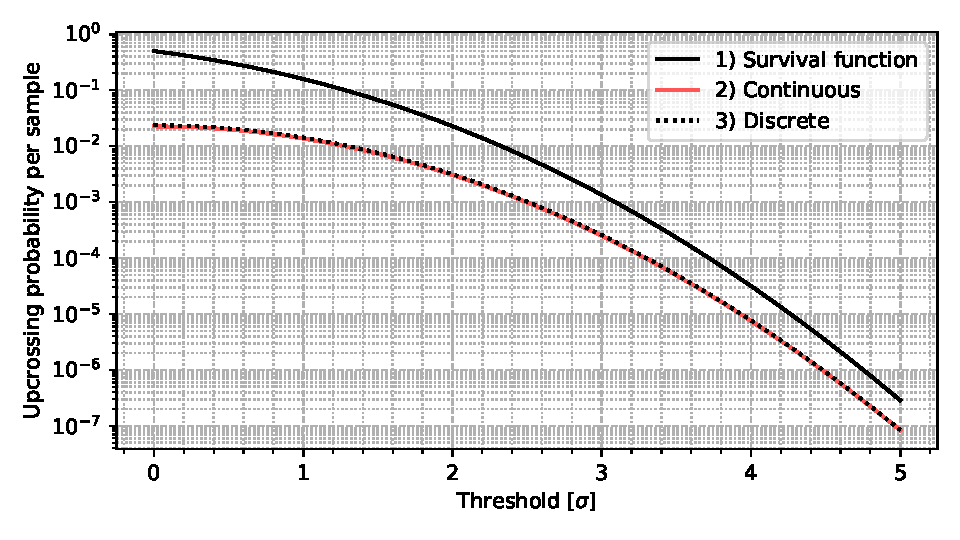
\includegraphics[width=1.00\textwidth]{figcrossingprob}

    \figcaption{crossingprob}{The threshold upcrossing rate expressed as
    per-sample crossing probability (i.e.\ the rate if the sampling frequency
    is~1) for an autocorrelated Gaussian waveform, estimated using three
    formulae: 1) the probability for a single sample to be higher than the
    threshold, 2) a formula for continuous processes (equation~\ref{eq:rcont}),
    3) an approximation of the discrete case (equation~\ref{eq:rdisc}).}
    
\end{figure}

\subsection{Dead time}

The part of the data acquisition system (DAQ) that will look for threshold
crossings are the digitizers. A digitizer can not do complicated processing, so
when the threshold is crossed, a fixed slice of waveform is sent to the front
end processing (FEP) for further analysis (identify multiple signals, locate
them precisely, use a better filter, etc.). So we are not interested in
threshold crossings that happen close to a previous crossing.

This means that we have a dead time $T$. We arbitrarily decide to use a
non-restartable dead time, i.e.\ a crossing that happens within $T$ of a
previous one is ignored only if the latter has not been ignored itself.

Assuming that the crossings are a Poisson process, the formula to correct a
rate $R$ for the effect of the dead time is \cite[120]{knoll2010}:
%
\begin{equation}
    R \mapsto \frac R {1 + RT}. \label{eq:deadrate}
\end{equation}

The crossings of a Gaussian process are not in general a Poisson process. We
just need one counterexample to show this. Consider the process with
autocovariance function $k(x)=\cos(x)$. This is positive definite because it is
a linear combination of external products: $\cos(x-y) = \cos x \cos y + \sin x
\sin y$. Since $\cos$ is orthogonal to $\sin$, they are the eigenfunctions, so
a realization of the process is a random linear combination of harmonic
functions, which means that it is a shifted cosine, so the crossings are
exactly periodic.

However, in practice we expect that there will just be a ``repulsion'' or
``attraction'' of crossings within the scale of the autocorrelation time, so
for low crossing rate the formula should work.

\section{Test}

We want to test formula~\eqref{eq:rcont} on actual electrical noise.

\subsection{Data}

We will use the Proto0 run 886, a baseline acquisition. Tiles 53, 57 and 59
(used in Proto0) will be also studied with LNGS data. Tile~15 just with LNGS.
The LNGS data files are:
%
\begin{verbatim}
FBK/NUV/MB2-LF-3x/NUV-LF_3x_53/nuvhd_lf_3x_tile53_77K_64V_6VoV_1.wav
FBK/NUV/MB2-LF-3x/NUV-LF_3x_53/nuvhd_lf_3x_tile53_77K_66V_7VoV_1.wav
FBK/NUV/MB2-LF-3x/NUV-LF_3x_57/nuvhd_lf_3x_tile57_77K_64V_6VoV_1.wav
FBK/NUV/MB2-LF-3x/NUV-LF_3x_59/nuvhd_lf_3x_tile59_77K_64V_6VoV_1.wav
LFOUNDRY/pre-production-test/TILE_15/LF_TILE15_77K_55V_0VoV_1.wav
LFOUNDRY/pre-production-test/TILE_15/LF_TILE15_77K_59V_2VoV_1.wav
LFOUNDRY/pre-production-test/TILE_15/LF_TILE15_77K_63V_4VoV_1.wav
LFOUNDRY/pre-production-test/TILE_15/LF_TILE15_77K_67V_6VoV_1.wav
LFOUNDRY/pre-production-test/TILE_15/LF_TILE15_77K_71V_8VoV_1.wav
LFOUNDRY/pre-production-test/TILE_15/LF_TILE15_77K_73V_9VoV_1.wav
\end{verbatim}

\marginpar{Expand and adapt this paragraph after chapter 3 is done.}

The Proto0 data is without signals so we use it as it is. For the LNGS data
we take the pre-trigger part of the events, and ignore events where any
pre-trigger sample is less than~750 (860 for tile~15).

We plot the time-value histogram of the data for tile 53 in Proto0 and LNGS
(figure~\ref{fig:hist2dtile53}), for tile 15 at maximum overvoltage, and for
tiles 57 and 59 (figure~\ref{fig:hist2dtile155759}).

\marginpar{No need for more explanations of the time-value histograms since
there will be some of them in chapter 3.}

\marginpar{Move the histograms to the end of the chapter.}

\begin{figure}
    
    \mbox{
    \hspace{-0.20\textwidth}
    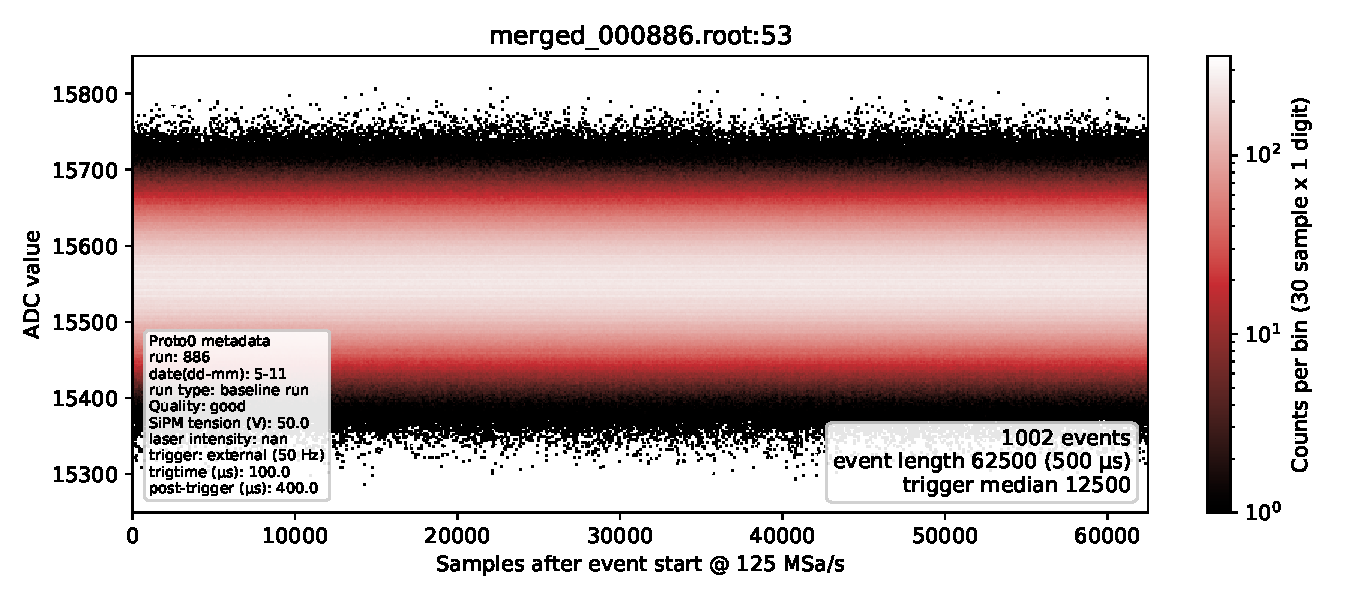
\includegraphics[width=1.41\textwidth]{fighist2dtile53-0}
    }
    \mbox{
    \hspace{-0.20\textwidth}
    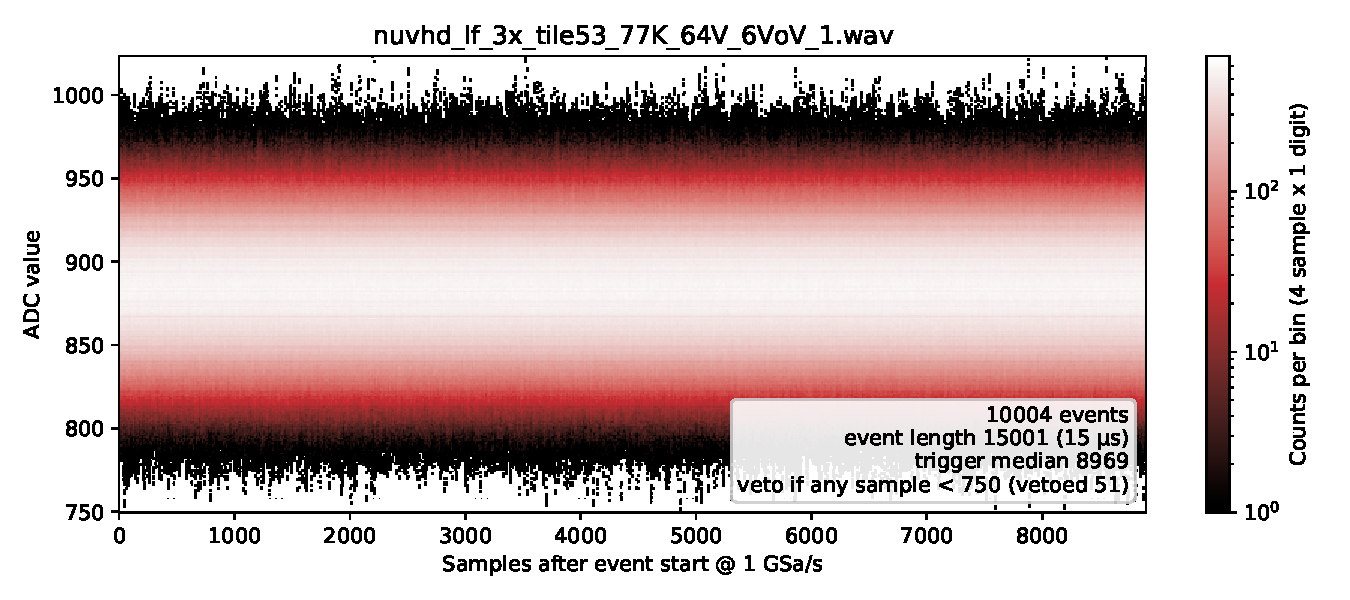
\includegraphics[width=1.41\textwidth]{fighist2dtile53-1}
    }
    \mbox{
    \hspace{-0.20\textwidth}
    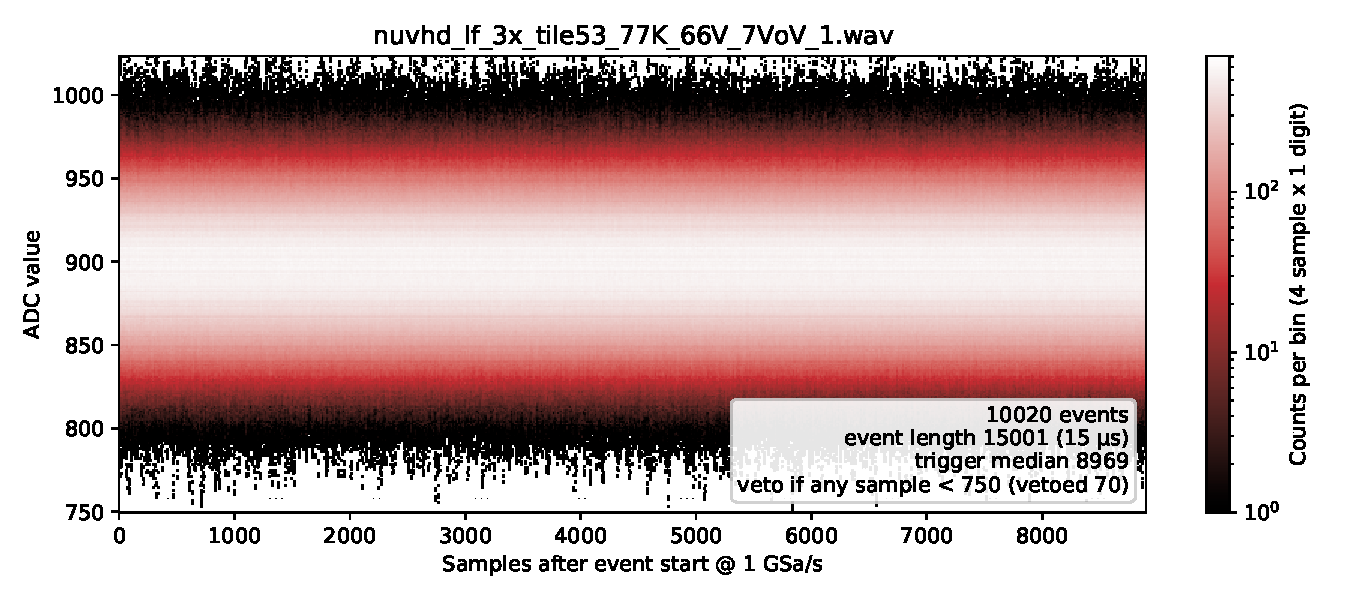
\includegraphics[width=1.41\textwidth]{fighist2dtile53-2}
    }
    
    \figcaption{hist2dtile53}{Time-value histograms of tile 53 noise in Proto0
    with a baseline acquisition, and in LNGS pre-trigger at overvoltage \SI6V
    and \SI7V.}
    
\end{figure}

\begin{figure}
    
    \mbox{
    \hspace{-0.20\textwidth}
    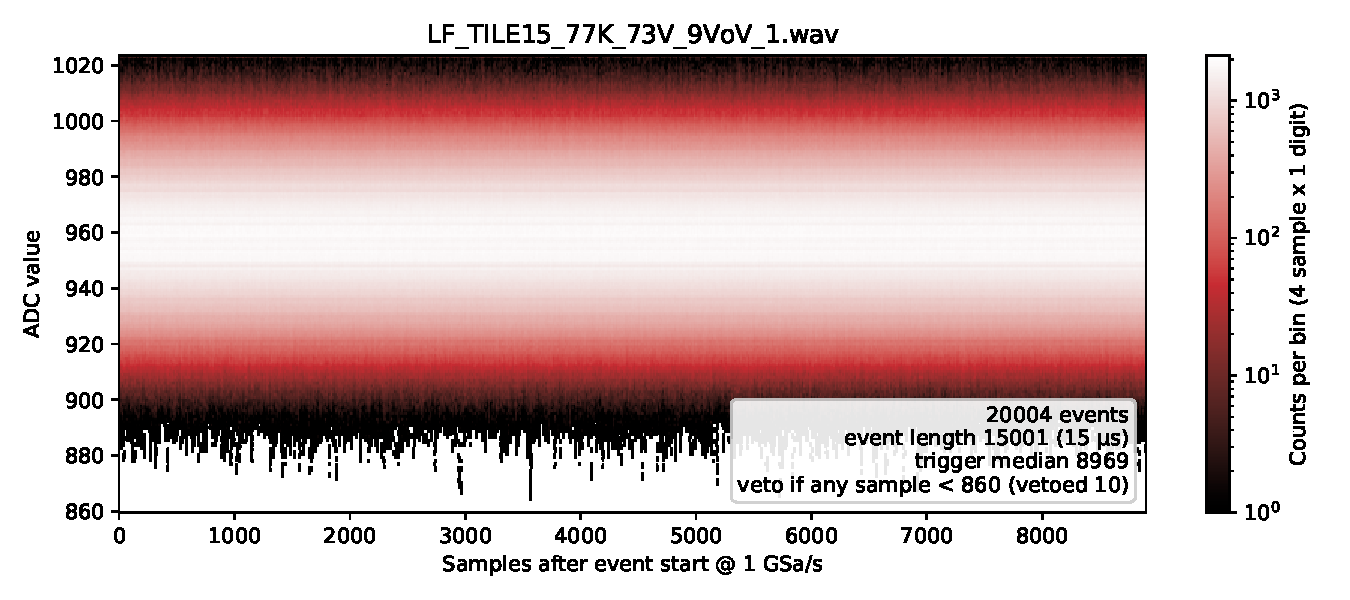
\includegraphics[width=1.41\textwidth]{fighist2dtile155759-0}
    }
    \mbox{
    \hspace{-0.20\textwidth}
    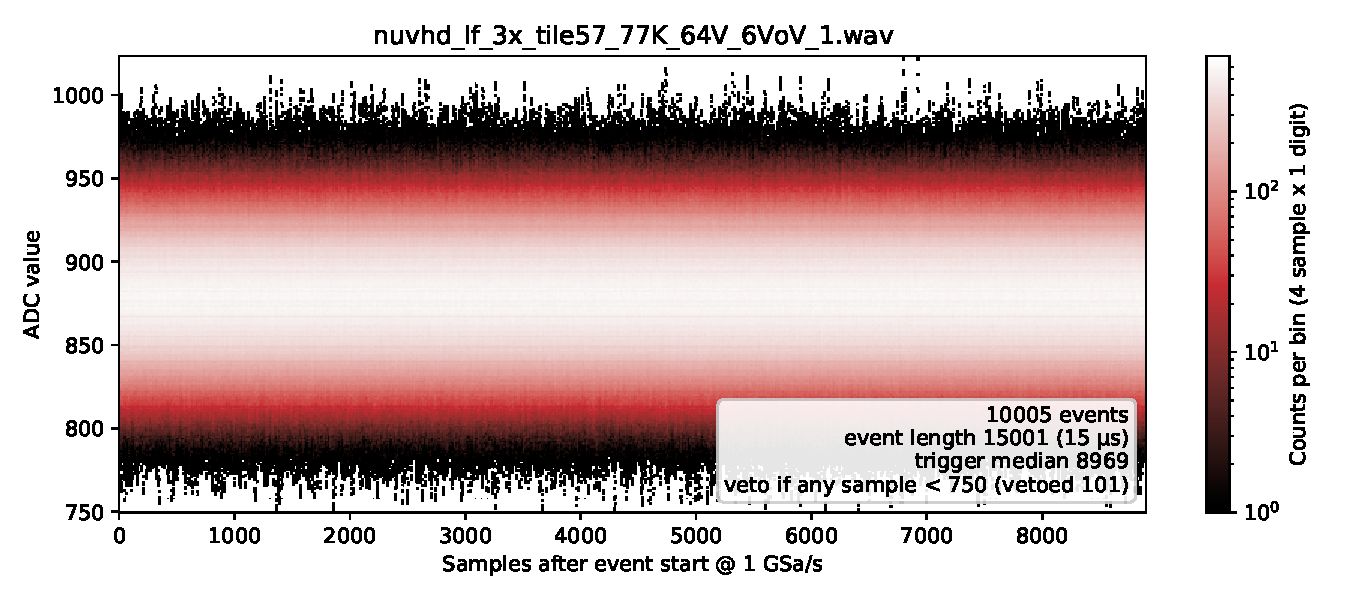
\includegraphics[width=1.41\textwidth]{fighist2dtile155759-1}
    }
    \mbox{
    \hspace{-0.20\textwidth}
    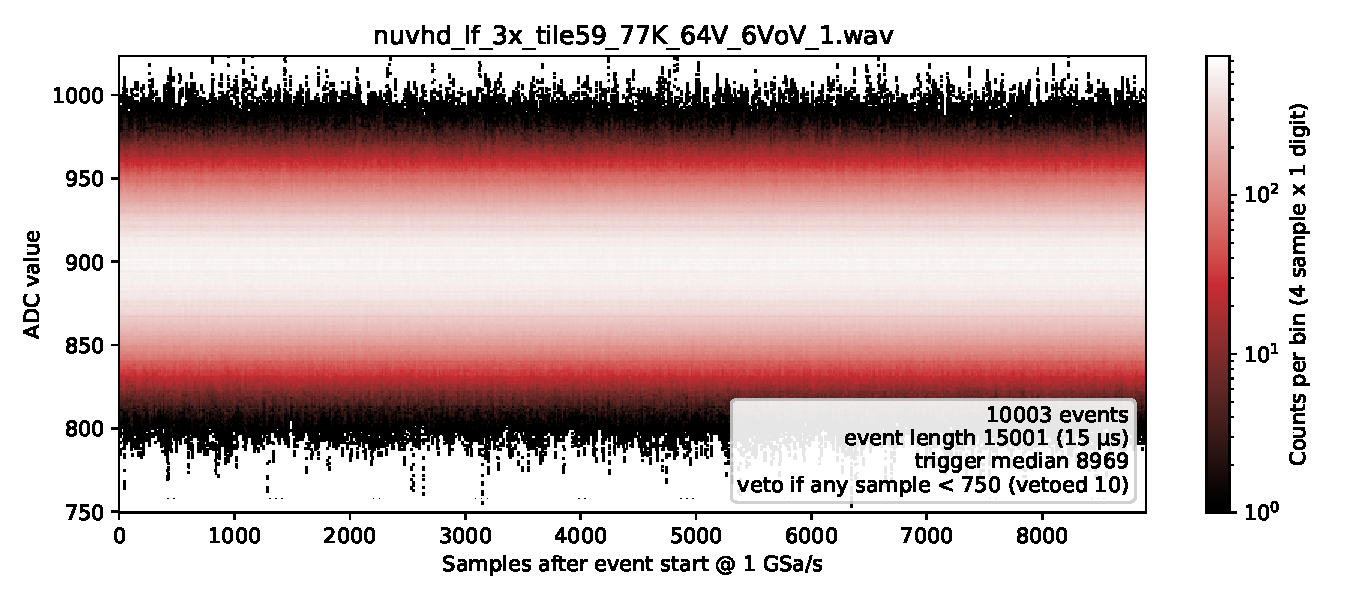
\includegraphics[width=1.41\textwidth]{fighist2dtile155759-2}
    }

    \figcaption{hist2dtile155759}{Time-value histograms of tiles 15, 57 and 59
    noise in LNGS data.}
    
\end{figure}

\subsection{Filter}

We filter using a \SI1{\micro s} moving average with \SI1{\micro s} of baseline
and \SI1{\micro s} of dead time, without delay between the baseline and the
signal averages. In figure~\ref{fig:sqfilt} we show an example filtered
waveform and the filter shape.

\begin{figure}

    \hspace{-0.20\textwidth}
    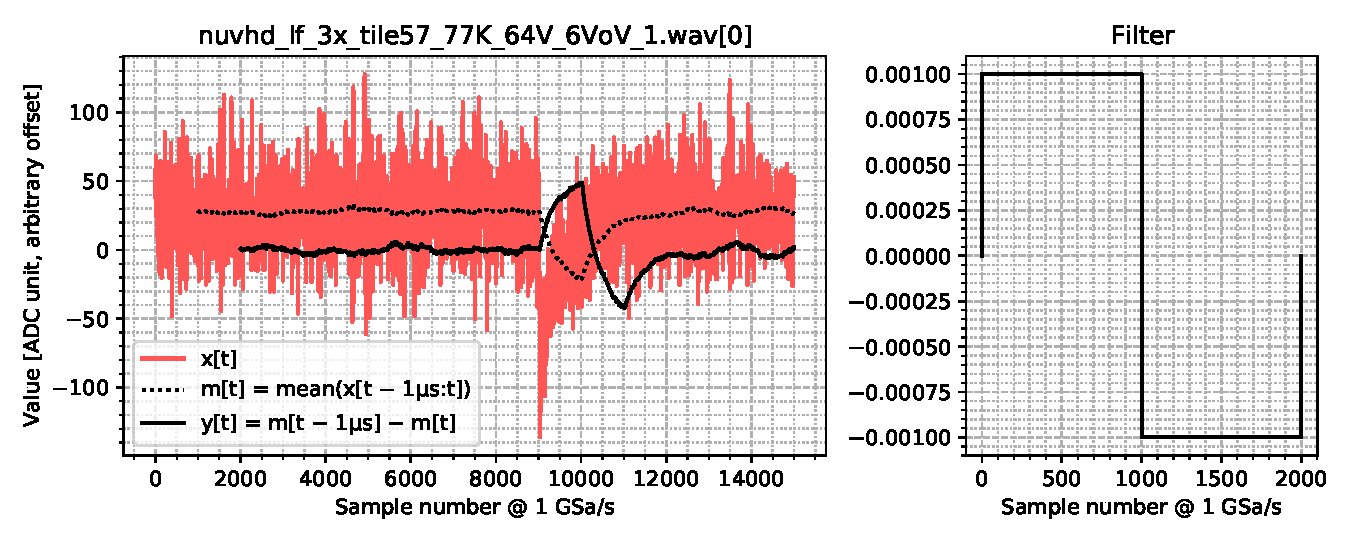
\includegraphics[width=1.41\textwidth]{figsqfilt}

    \figcaption{sqfilt}{A filtered waveform. The computation is split into a
    moving average $m$ (dotted line) and its finite difference $y$ (solid black
    line). The right plot shows the overall filter shape. (We use an event with
    a signal just to see how the filter behaves, the analysis is done on noise
    only.)}

\end{figure}

From chapters~\ref{ch:snr} and~\ref{ch:timeres} we know this is not the optimal
filter by SNR neither by temporal resolution. However since we don't know which
filter will be used it is appropriate to make a conservative choice.

Since on LNGS data the events are short compared to the filter length
(\SI9{\micro s} vs. \SI2{\micro s}), we need to take into account boundary
effects. The output length of the filtered waveform is $(\text{initial length})
- \SI2{\micro s} + \SI1{sample}$; to compute the rate we have to divide by this
quantity instead of the initial waveform length.

The dead time does not play nicely with borders, because a hypothetical unseen
crossing within \SI1{\micro s} before the event start could kill a crossing in
the event. Moreover, at low thresholds, the first crossing will happen
almost immediately, and again immediately after the dead time ends, thus the
number of crossings per event is quantized.

A complete solution to these problems would be to avoid counting the crossings
which happen within \SI1{\micro s} after the event start (although they are
detected and do project a dead time on the following ones), and in the
remaining region further select a subregion which is \SI1{\micro s} shorter but
has a uniformly random starting position.

However we care only about low rates, and at low rate the dead time boundary
effects are negligible, so we will keep the whole filtered region.

\subsection{Algorithm}

The simplest way to count the threshold crossings as a function of the
threshold is to repeat the calculation varying the threshold. The computational
complexity is $O(nN)$ where $n$ is the number of thresholds and $N$ the number
of samples.

To produce a smooth curve (large $n$) we use instead a reverse histogram. We
choose an evenly spaced range of thresholds. For each pair of consecutive
samples, if the second sample is higher than the first, we determine the
subrange of thresholds that falls between the samples, and increment their
counts. To apply the dead time, we keep a per-threshold last occurence time.

Since the range of thresholds is evenly spaced, the subrange can be found
arithmetically, so the complexity is just $O(N)$, it does not depend on the
number of thresholds.

\subsection{Results}

In figure~\ref{fig:fakerate1} we compare the measured threshold crossings with
the continuous-derived formula~\eqref{eq:rcont} for a single tile over the
entire threshold range. The coefficients $\sigma$ and $k_2$ for the formula are
computed on each filtered event and then averaged. Finally, the dead time is
accounted for with~\eqref{eq:deadrate}. For the data, the conversion from count
to rate is done dividing by the length of the filtered waveform (so \SI2{\micro
s} less than the initial length per event).

The agreement is decent at low and high rates, less so in an intermediate
region. The agreement at high rate is probably a sort of saturation due to dead
time, since the maximum rate allowed by dead time is $1/(\SI1{\micro s}) =
\SI1{Mcps}$. Keep into account that the scale is logarithmic, so even where the
lines are closer they still differ by a factor~1.3, while the Poisson error is
approx.~\SI3\% since the count is~1000.

\begin{figure}
    
    \hspace{-0.11\textwidth}
    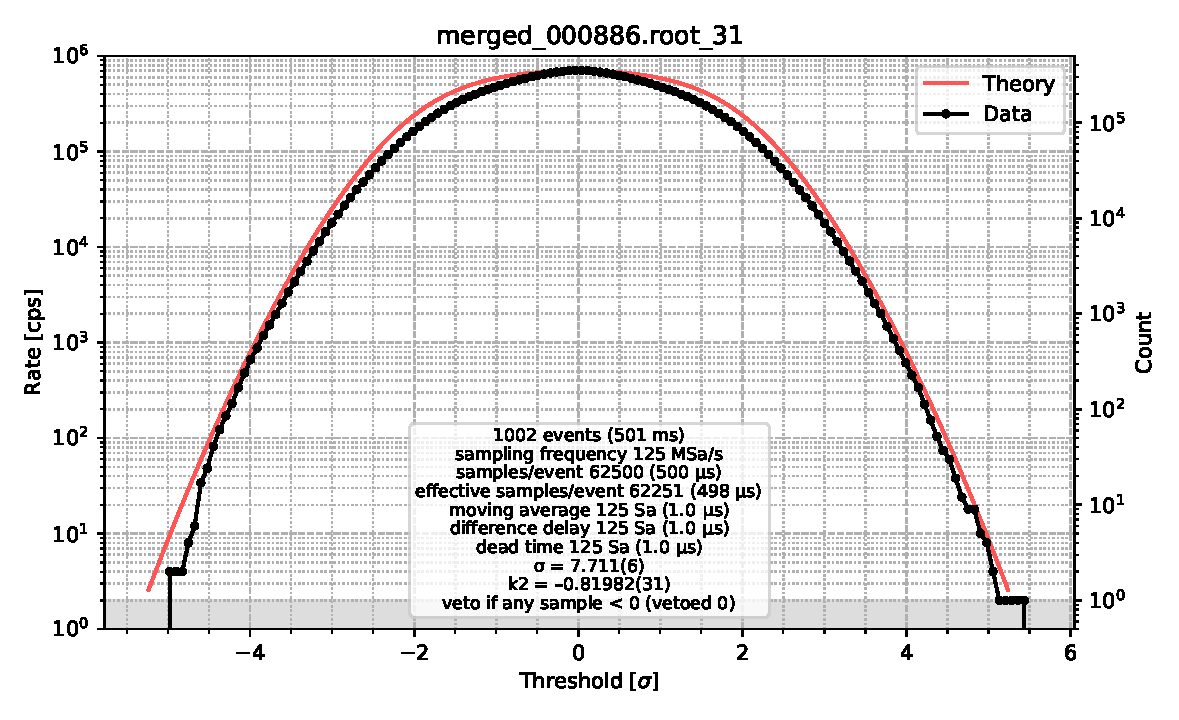
\includegraphics[width=1.23\textwidth]{figfakerate1}

    \figcaption{fakerate1}{Measured and predicted fake rate for tile~31 in
    Proto0 with a noise-only acquisition. The right scale shows the actual
    count of threshold crossings for the data, with a gray band marking one
    crossing.}
    
\end{figure}

\marginpar{Add reference to the formula in figure~\ref{fig:fakerate1}.}

In figure~\ref{fig:fakerate} we show the same comparison together for all
datasets, divided in three groups (tile~15 LNGS data, Proto0 data, LNGS other
tiles). The parameters for the formula, and the rates at threshold~$4\,\sigma$,
are listed in table~\ref{tab:fakerate}.

In the second group above some threshold the measured rate stops decreasing and
remains constant at approximately 10 counts. This is probably due to pulses
which our very simple veto can not filter away, we guess 1 pe dark/random
pulses.

In figure~\ref{fig:fakerate} we highlight the measured rates for tile~53
because they are evident outliers. The rate remains higher than the theory
predicts and than the other tiles as the threshold increases. This is visibile
in Proto0, and in LNGS at \SI6{VoV}, but not at \SI7{VoV}.

Analogously, from table~\ref{tab:fakerate} we see that the quantity $f_s
\sqrt{-k_2}/(2\pi\sigma)$ that multiplies the exponential in~\eqref{eq:rcont}
is different from the others for tile~53, in the same cases as the data, but
with the opposite trend. This variation seems to depend only on an increase in
$\sigma$ and not on $k_2$.

Even though it's weird that this problem disappears at \SI7{VoV}, it can't be a
coincidence that it arises for the same tile in different setups, showing up
both as an increased noise RMS and an higher threshold crossing rate, so it
must be some property of the tile itself.

Comparing the 2D histograms for tile~53 (figure~\ref{fig:hist2dtile53}) to the
others (figure~\ref{fig:hist2dtile155759}) there is no apparent difference.
Three possible explanations come to mind: 1) a violation of Gaussianity, 2)
stray pulses, 3) electrical noise.

Regarding Gaussianity, we checked the distribution of the samples before
filtering and it agrees very well with a Gaussian. If they are stray pulses,
they do not have the same height, otherwise they would show up as a flat rate
curve. It could be electrical noise with a frequency of approx.~$1/(\SI2{\micro
s}) = \SI{500}{kHz}$, since our filter would be very good at picking that up.

\marginpar{Looking at the spectrum it is evident that there's a very low
frequency component ($<\SI{10}{kHZ} = 1/(\SI{100}{\micro s})$) absent in other
tiles. Maybe they are sudden changes of baseline? I should look at events where
crossings with high threshold happen.}

\begin{table}
    
    \hspace{-0.16\textwidth}
    \begin{tabular}{
        c
        S[table-format=2]
        S[table-format=>1]
        S[table-format=3]
        S[table-format=2.1]
        S[table-format=+1.4]
        S[table-format=2.3]
        S[table-format=1.1]
        *2S[table-format=1.2]
    }
        \toprule
        \multicolumn3c{Data}
        &
        &
        &
        &
        &
        & \multicolumn2c{Rate @ $4\,\sigma$} \\
        \cmidrule(r){1-3} \cmidrule(r){9-10}
        
        Setup
        & {Tile}
        & {Overvoltage}
        & {$T$}
        & {$\sigma$}
        & {$k_2$}
        & {$\operatorname{Std}[\bar{k_2}]\sqrt T$}
        & {$f_s \sqrt{-k_2}/(2\pi\sigma)$}
        & {Theory}
        & {Data} \\
        
        &
        & {[\si{V}]}
        & {[\si{ms}]}
        & {[\si{u}]}
        & {[\si{u^2}]}
        & {[\si{u^2 ns^{1/2}}]}
        & {[\si{Mcps}]}
        & {[\si{kcps}]}
        & {[\si{kcps}]} \\
        \midrule
        
  LNGS & 15 &  0 & 138 &  1.6 & -0.0017 & 0.012 & 4.2 &  1.4 &  1.1 \\
  LNGS & 15 &  2 & 138 &  1.5 & -0.0017 & 0.012 & 4.3 &  1.4 &  1.2 \\
  LNGS & 15 &  4 & 138 &  1.5 & -0.0017 & 0.012 & 4.3 &  1.4 &  1.3 \\
  LNGS & 15 &  6 & 138 &  1.5 & -0.0017 & 0.012 & 4.4 &  1.5 &  1.1 \\
  LNGS & 15 &  8 & 138 &  1.5 & -0.0017 & 0.012 & 4.5 &  1.5 &  1.4 \\
  LNGS & 15 &  9 & 138 &  1.4 & -0.0017 & 0.012 & 4.6 &  1.5 &  1.3 \\  \midrule
  LNGS & 53 &  6 &  69 &  3.8 & -0.0044 & 0.030 & 2.7 & 0.92 &  2.6 \\
  LNGS & 53 &  7 &  69 &  2.1 & -0.0043 & 0.029 & 5.0 &  1.7 &  1.0 \\
  LNGS & 57 &  6 &  68 &  2.2 & -0.0043 & 0.031 & 4.8 &  1.6 &  1.2 \\
  LNGS & 59 &  6 &  69 &  2.2 & -0.0040 & 0.028 & 4.6 &  1.5 &  1.0 \\  \midrule
Proto0 & 29 & <0 & 499 &  8.3 &   -0.86 &   10. & 2.2 & 0.74 & 0.77 \\
Proto0 & 30 & <0 & 499 &  6.9 &   -0.75 &   6.0 & 2.5 & 0.84 & 0.67 \\
Proto0 & 31 & <0 & 499 &  7.7 &   -0.82 &   7.0 & 2.3 & 0.78 & 0.60 \\
Proto0 & 32 & <0 & 499 &  7.0 &   -0.76 &   6.6 & 2.5 & 0.83 & 0.67 \\
Proto0 & 34 & <0 & 499 &  6.5 &   -0.78 &   6.2 & 2.7 & 0.90 & 0.62 \\
Proto0 & 36 & <0 & 499 &  7.7 &   -0.84 &   7.1 & 2.4 & 0.79 & 0.63 \\
Proto0 & 37 & <0 & 499 &  6.5 &   -0.69 &   5.4 & 2.5 & 0.85 & 0.67 \\
Proto0 & 38 & <0 & 499 &  7.7 &   -0.84 &   7.1 & 2.4 & 0.80 & 0.59 \\
Proto0 & 39 & <0 & 499 &  7.6 &   -0.91 &   7.5 & 2.5 & 0.84 & 0.68 \\
Proto0 & 41 & <0 & 499 &  7.5 &   -0.87 &   7.1 & 2.5 & 0.83 & 0.71 \\
Proto0 & 42 & <0 & 499 &  7.0 &   -0.82 &   6.8 & 2.6 & 0.87 & 0.63 \\
Proto0 & 52 & <0 & 499 &  7.8 &   -0.82 &   6.5 & 2.3 & 0.77 & 0.61 \\
Proto0 & 53 & <0 & 499 & 10.1 &   -0.90 &   8.0 & 1.9 & 0.63 &  2.3 \\
Proto0 & 54 & <0 & 499 &  8.0 &   -0.89 &   7.4 & 2.4 & 0.79 & 0.59 \\
Proto0 & 55 & <0 & 499 &  8.0 &   -0.85 &   7.1 & 2.3 & 0.77 & 0.63 \\
Proto0 & 57 & <0 & 499 &  7.8 &   -0.88 &   7.4 & 2.4 & 0.80 & 0.69 \\
Proto0 & 58 & <0 & 499 &  7.6 &   -0.82 &   6.4 & 2.4 & 0.79 & 0.65 \\
Proto0 & 59 & <0 & 499 &  7.6 &   -0.79 &   6.6 & 2.3 & 0.77 & 0.55 \\
Proto0 & 60 & <0 & 499 &  7.5 &   -0.77 &   6.3 & 2.3 & 0.78 & 0.61 \\
Proto0 & 61 & <0 & 499 &  8.0 &   -0.89 &   7.4 & 2.4 & 0.79 & 0.60 \\
Proto0 & 62 & <0 & 499 &  7.6 &   -0.80 &   6.6 & 2.3 & 0.78 & 0.62 \\
Proto0 & 63 & <0 & 499 &  8.1 &   -0.86 &   7.1 & 2.3 & 0.76 & 0.61 \\
Proto0 & 64 & <0 & 499 &  7.9 &   -0.81 &   6.9 & 2.3 & 0.76 & 0.66 \\
Proto0 & 65 & <0 & 499 &  7.5 &   -0.80 &   6.4 & 2.4 & 0.80 & 0.62 \\
Proto0 & 66 & <0 & 499 &  8.2 &   -0.91 &   7.5 & 2.3 & 0.77 & 0.61 \\
        
        \bottomrule
    \end{tabular}
    
    \tabcaption{fakerate}{The coefficients measured on the filtered waveforms
    needed to evaluate the formula for the threshold upcrossing rate. $T$ is
    the total duration, $\sigma$ the standard deviation, $k_2$ the covariance
    of the waveform with its second derivative (equation~\ref{eq:k2}),
    $\operatorname{Std}[\bar{k_2}]$ the uncertainty on the value of $k_2$
    determined as the standard deviation of the sample mean of $k_2$ values
    across events. The unit ``\si{u}'' is the ADC digit.}
    
\end{table}

\begin{figure}
    
    \hspace{-0.12\textwidth}
    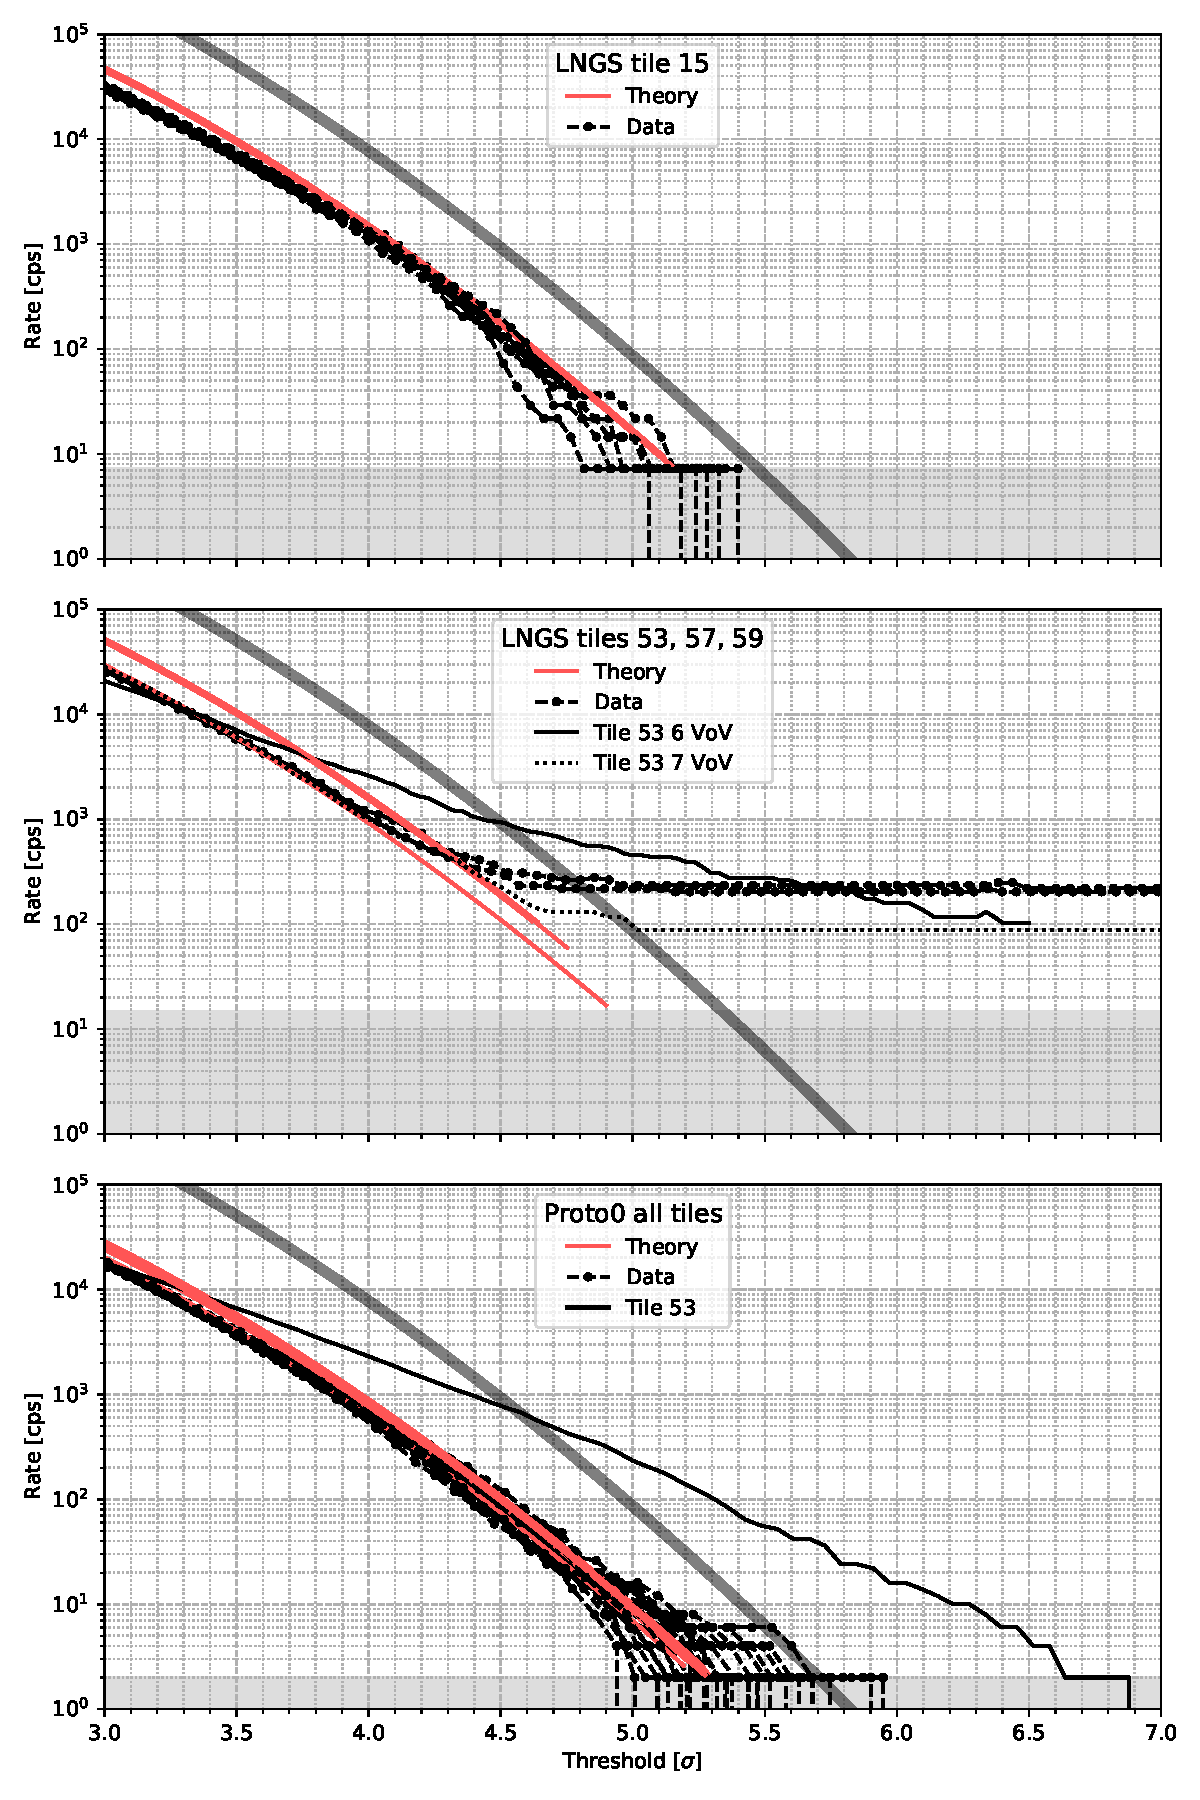
\includegraphics[width=1.25\textwidth]{figfakerate}
    
    \figcaption{fakerate}{The threshold upcrossing rate both counting directly
    the crossings on data and computing it with formula~\eqref{eq:rcont}. The
    gray band marks the rate corresponding to a single crossing counted in the
    data.}
    
\end{figure}

We didn't investigate further the discrepancy for tile~53. Anyway, for all
other tiles we looked at it works well enough.

We now want to estimate the minimum amount of data required for the procedure.
From table~\ref{tab:fakerate} we see that the relative error on $k_2$ times the
square root of the time, $C \equiv
\operatorname{Std}[\bar{k_2}]\sqrt{T}/|k_2|$, is approximately \SI8{ns^{1/2}}
in all cases. The error should be proportional to $T^{-1/2}$, so to have an
\SI1\% error we need $T_{\SI1\%} = (100 C)^2 = \SI{0.7}{ms}$.

For convenience we summarize all the steps to compute the fake rate:
%
\begin{enumerate}
    
    \item Acquire \SI1{ms} of noise data.
    
    \item Filter the data (including baseline subtraction) producing a
    filtered waveform $\mathbf y$.
    
    \item Compute the standard deviation $\sigma$ and $k_2 =
    \operatorname{Cov}[y_i, y_{i+1} + y_{i-1} - 2y_i]$.
    
    \item Compute the fake rate for threshold $u$ using $r =
    f_s\sqrt{-k_2/(2\pi)}\operatorname{gauss}(u;0,\sigma)$ where $f_s$ is the
    sampling frequency.
    
\end{enumerate}
%
The probability of the formula not working due to mysterious reasons is \SI4\%.
If it works, the uncertainty for low rate is \SI{\pm50}\% and the result is an
overestimate with probability \SI{90}\%. (These assessments are based on
table~\ref{tab:fakerate} but are somewhat subjective.)

Alternatively, if one has a noise spectrum available but not the noise
waveform, obtain the autocovariance by doing the discrete Fourier transform of
the power spectrum \cite[84]{ferrante2015} and then normalizing it to be
$\sigma^2$ in 0. Then $k_2$ is obtained by the covariance at lag 1 $c$ with
\eqref{eq:c2k2}. (If the spectrum was obtained from the discrete Fourier
transform of a noise waveform, $c$ is the first coefficient after the central
one in the autocovariance.)
